\chapter{Grafiken\index{Grafiken}}\label{sec:grafiken}
\section{Wichtigste Punkte}
\begin{itemize}
	\item Schematische Darstellungen sollten wenn irgendmöglich vektoriell sein.
		Anstatt Screen\-shots wenn möglich als pdf <<drucken>> und dann das pdf
		vektoriell bearbeiten (z.B. mit Inkscape oder LibreOffice).
	\item In Graphen sind alle Achsen beschriftet, inkl. Masseinheiten.
	\item Sämtliche Zahlen müssen erklärt sein, entweder direkt in der Grafik
		oder in der Legende dazu.
	\item Jede Grafik wird mit einer Legende (<<$\backslash$caption>>) und einem
	<<$\backslash$label>> versehen. Dadurch erhält jede Grafik eine Nummer und wird
	automatisch im Abbildungsverzeichnis (<<$\backslash$listoffigures>>) aufgeführt.
%
	\item Jede Grafik muss im Text erwähnt werden (<<$\backslash$autoref>>).
\end{itemize}

\begin{wrapfigure}{r}{0.6\textwidth}
	\centering
	\includegraphics[width=0.55\textwidth]{wrapfig-code.pdf}
	\captionof{figure}{Code für die \autoref{fig:wrapfig}.}
	\label{fig:wrapfig}
\end{wrapfigure}


\LaTeX{} platziert die Grafik nicht unbedingt dort, wo man es
erwartet. Abhilfe kann da z.B. <<wrapfigure>> bieten.

Dieser Paragraph ist ein Beispiel dazu, der nötige 
\LaTeX-Code ist in der \autoref{fig:wrapfig} zu finden.


\section{Vektorgrafiken}
Ideal sind Vektorgrafiken (.pdf oder .svg Formate). Diese können über
Umwege auch unter Windows produziert werden:
\begin{itemize}
\item Erstellen Sie Ihre Grafik mit einem Programm (aber nicht ein
  Pixelbasiertes Programm wie z.B. Paint, Gimp oder Photoshop),
  sondern z.B. Excel oder Powerpoint. Konvertieren Sie dann die Grafik
  ins pdf-Format, indem Sie einen <<pdf-Drucker>> installieren und die
  Grafik darauf <<ausdrucken>>.
\item Sie können aber auch OpenOffice Calc/Draw oder Inkscape
  verwenden. Diese frei verfügbaren Programme können direkt im
  .pdf-Format oder .svg-Format speichern.
\item Bearbeiten Sie dann die Grafiken, falls nötig, mit Inkscape
  (frei verfügbar).
\end{itemize}

\subsection{Vektorielle Screenshots von Webseiten}
Als pdf Drucken, danach in Inkscape bearbeiten.

Wenn man möchte, dass die Seite aussieht wie auf dem Bildschirm,
kann in Chrome wie folgt vorgegangen werden:
\begin{itemize}
	\item Entwicklertools öffnen (F12).
	\item Im Hamburgermenu <<More Tools>> $\leftarrow$ <<Rendering>>
	\item Emulate Rendering type: <<screen>>.
	\item Dann <<ausdrucken als pdf>>.
	\item pdf nötigenfalls bearbeiten.
\end{itemize}

\section{Einbinden einer Grafik}

\begin{figure}[ht] % try placing 'h'ere, then 't'op of next page
    \centering
    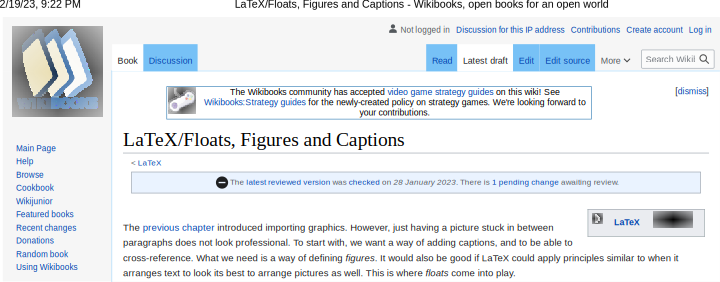
\includegraphics[width=0.8\textwidth]{wikibooks-figures.pdf}
    \caption[Wikibooks]{Screenshot der Wikibooks website \cite{figures}. Beachten
        Sie, dass der Text in dieser Grafik sogar selektierbar ist.}
    \label{fig:wikibooks}
\end{figure}

Dazu muss gar nicht viel gesagt, weil schon alles
auf Wikibooks \cite{figures} gefunden werden kann, 
wovon in \autoref{fig:wikibooks} ein
Screenshot zu sehen ist. Der \LaTeX-Code ist in 
\autoref{lst:figure-example} zu finden.

\subsection{\LaTeX-Code}
Zum Einbinden der \autoref{fig:wikibooks}
wurde der \LaTeX-Code im Listing 
\ref{lst:figure-example} verwendet.

\lstinputlisting[
label=lst:figure-example,
language=tex,
caption={Code zum Einbinden der \autoref{fig:wikibooks}.},
]{graphics-figure-example.tex}
